% !TEX root = ../thesis.tex
\chapter{Survey management}
\label{chapter:<survey_management>}

\section{Introduction}
\label{sec:survey_management_introduction}

In this chapter we will analyze, in depth, how to perform, create and add a new type of survey in the system. Movish is indeed a complex system that can be used as a plain movie catalog or as a survey system. When in survey mode, the system changes smoothly the layout in order to guide the user through the questions and removes many not useful links that would bring the user out of the application or in some undefined states that are only valid when browsing the catalog without performing a survey.

Guiding a user while performing a survey is a challenge. The survey must be designed such that the user doesn't waste time in not useful operation but it is still free to browse, search and rate any content the user wants in order of not alter the recommendation. The user must be guided in order to focus his/her attention in what is the survey goal also. This makes planning a new type of survey a challenge and a task that requires a lot of thinking before being able to implement one. 

Movish simplifies the process of adding a new type of survey, that i exposed in secion \ref{sec:adding_new_survey_type_to_Movish} while survey creation is exposed in section \ref{sec:survey_creation} with the two types of survey supported, the algorithm performance and the algorithm strength.

\section{Survey creation}
\label{sec:survey_creation}

The creation of a survey is the action of adding a survey to the system and perform all the necessary operations that make the system able to accept new user or existing ones to perform the survey. A user with administration privileges is needed to make a new survey. After logged in the user has to go to the admin interface explained in secion \ref{sec:admin_interface}.

\begin{figure}
  \centering
  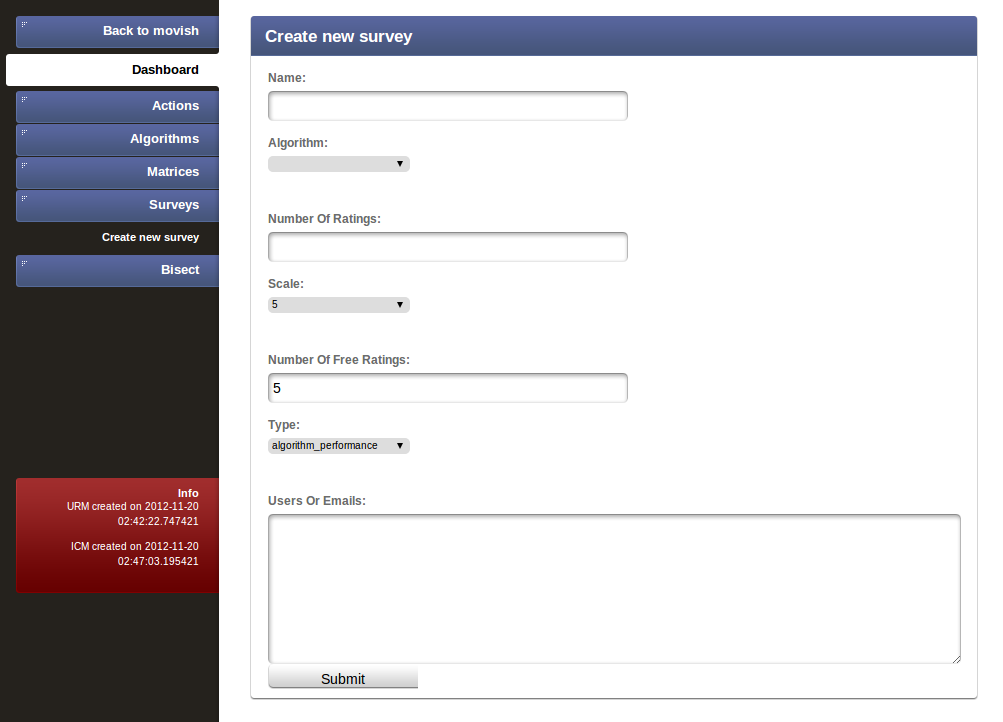
\includegraphics[width=\textwidth]{figures/survey_creation.png}
  \caption{Survey creation}
  \label{fig:survey_creation}
\end{figure}

Figure \ref{fig:survey_creation} shows the form to create a new survey. The administrator has to pick up a name, an algorithm name (from the list), a number of ratings representing the number of ratings that will be displayed to the user while being in the recommendation part of a survey; the scale of the rating, the number of free ratings the user is able to perform before receiving the recommendation; the survey type that can be \textbf{algorithm\_performance} or \textbf{algorithm\_strength}. We will talk about these two types in the next subsections. The administrator can optionally add a set of comma separated emails of the user that will be notified with a mail that there is a survey for them. Users that are not in the system will be added and a mail will be sent as well. After submitting the form the task of creating a new survey is created. 

In general, any user can perform the surveys that are in the system if the user knows the id of the survey. The entry point for each user is in fact \textit{survey/demographic/ID} where ID is the id of the survey. The user must be logged in to access that resource. In the case the user is not registered, it has to register first. To remove this additional step which is mandatory for the recommendation engine to work but may be a problem for a user that is just on the site to perform a survey a special handler that creates a user to the system and start the survey has been created. It can be accessed from \textit{http://movish.co/survey/amazonturk/ID} where ID is the id of the survey. The administrator can see the id of the survey looking at the last number of the \textit{amazon turk link} column in the survey menu in figure \ref{fig:surveys_menu}.

Users have not be bounded to a particular survey in order to allow the administrator to select other users while the survey in progress and to allow the Amazon Mechanical Turk \cite{amazon-mechanical-turk} cooperation. We will talk more about amazon mechanical turk on secion \ref{sec:crowdsourcing}. As for now the reader can think of amazon mechanical turk as a service offered by amazon to provide human workforce for tasks that are able to be performed with a computer. Online surveys are a typical case of this kind of work.

Result of the surveys can be retrieved in the survey admin page shown in figure \ref{fig:surveys_menu}. Clicking on the small icon with a pencil with a label of \textit{download result} the administrator can get the results of the survey in \ac{csv} format.

\begin{figure}
  \centering
  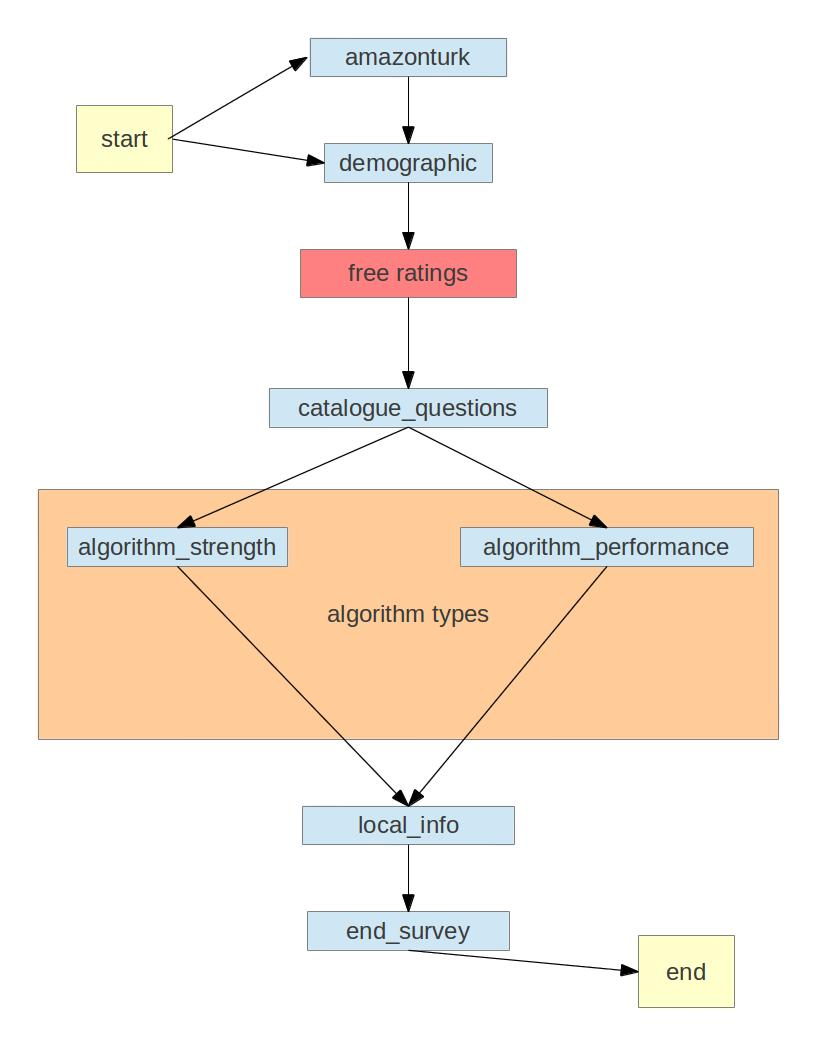
\includegraphics[width=\textwidth]{figures/movish_survey_architecture.jpg}
  \caption{Survey architecture: relation between functions}
  \label{fig:survey_architecture}
\end{figure}

Figure \ref{fig:survey_architecture} shows the survey subsystem architecture. The user starts from the \textbf{start} box and ends in the \textbf{end} box. The start can happen from the \textit{amazonturk} link ad described earlier or by direct invite at survey creation, in that case the user goes directly to \textbf{demographic}. After filling the form the user is redirected in a modified homepage without the possibility to logout and without a the main slider with only the possibility to surf the catalog and search for movies. This step is called \textbf{free ratings} and the user has to rate the number of ratings that the admin specified as \textit{number of free ratings} in survey creation. After the user has to answer a series of question regarding the catalogue. This phase is performed by the function \textbf{catalogue\_questions}. From now the behaviour of the system depends from the type of survey. As for now two types of surveys are implemented and they are performed by \textbf{algorithm\_strength} and \textbf{algorithm\_performance} respectively. \textbf{catalogue\_questions} is able to fetch the survey type and redirect the user to the correct page generated by the correct survey type. All survey types, after performing the recommendation must redirect to the \textbf{local\_info} function that take cares of asking the last questions to the user and redirect him/her to the \textbf{end\_survey} page. The end survey page exposes the Amazon Mechanical Turk confirmation code that the user has to submit to the amazon form in order to claim the survey that is just being completed. 

\subsection{Algorithm performance}
\label{sec:algorithm_performance}

Algorithm performance is the first type of survey that has been implemented. It shows the recommendation to the user displaying one movie at time and asking him/her subsequent questions. The questions that the user answers are contextual, it means that they vary depending from the previous questions. The main goal is to give to the user all the information in order to make him/her able to rate the movie even if he/she did not actually watched the movie.
This was the first type of survey and the only one implemented in Milo \cite{thesis-andreia}. The flow chart in figure \ref{fig:algorithm_performance_flow_chart} shows the questions that the user has to answer and their order.

\begin{figure}
  \centering
  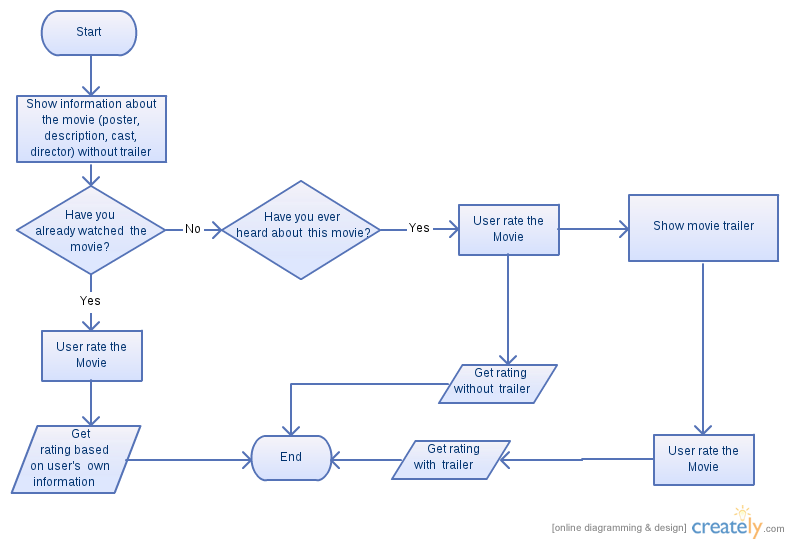
\includegraphics[width=\textwidth]{figures/algorithm_performance_flow_chart.png}
  \caption{Algorithm performance flow chart}
  \label{fig:algorithm_performance_flow_chart}
\end{figure}

The user starts from the \textbf{start} box and ends at the \textbf{end} box. As the reader can verify the user may not answer all the questions or get all the information before getting to the \textbf{end} box.

\subsection{Algorithm strength}
\label{sec:algorithm_strenght}

Algorithm strength is the second type of survey that Movish supports. It has been deployed to perform the research of chapter \ref{chapter:<research_number_of_items>}. In this type of survey the user gets a recommendation and the user can see the first Nth elements where N is the \textit{number of ratings} that the administrator set at survey creation. The system then asks some question about the recommendation to the user, the questions are:

\begin{itemize}
\item How many movies in this list have you ever watched?
\item How many movies in this list have you never heard of?
\item From the movies in this list that you have already watched, if any, how many do you like?
\item From the movies in this list that you have already watched, if any, how many do you dislike? (leave 0 if no one)
\item From 1 (low interesting) to 5 (very interesting) how interesting did you find the given recommendations?
\item How many movies in this list will you likely watch in the future?
\end{itemize}

This kind of survey is used to test how the perception of a good recommendation relates with the number of item shown to the user in order to understand how strong is an algorithm and in general how the number of items displayed to the user influences his/her perception of a good recommendation.  

\section{Adding new survey type to Movish}
\label{sec:adding_new_survey_type_to_Movish}

Adding a new survey to the system is a easy task which needs a bit of understanding in how the movish system works. Movish support a set of predefined questions that are the same for each survey and a variable set of questions and recommendation pages that can be composed and chained easily by the administrator. All the survey subsystem is defined in \textit{controllers/survey.py}. Each survey page is generated by three steps:

\begin{itemize}
\item \textbf{form definition}. Where the form that the user has to answer is defined using web2py \cite{web2py} helpers. Web2py helpers are function that produce a html code snippet accordingly. They are used to generate html on the controller or in the view itself.
\item \textbf{form submission}. Where the form that the user answered get submitted and saved in a database.
\item \textbf{data retrieval}. Where the data that is shown to the user during a particular survey page is retrieved.
\end{itemize}

Figure \ref{fig:algorithm_strength} shows how the \textit{algorithm\_strength} survey type is implemented. It shows clearly where the different parts of the survey page are composed. The first 13 lines, from 192 to 206 are for data retrieval. In those lines the recommendation for the given algorithm of the survey is retrieved. If there is no recommendation available for the current user in the given algorithm a new recommendation is scheduled and the system waits 5 seconds before reloading the same page and check that there is a recommendation. Lines from 207 to 215 are for form definition. The form is mainly formatted with a table in which there are select fields. The \textit{\_name} property is very important because it defines the name that will be displayed when the administrator retrieves the survey results.  

\begin{figure}
  \centering
  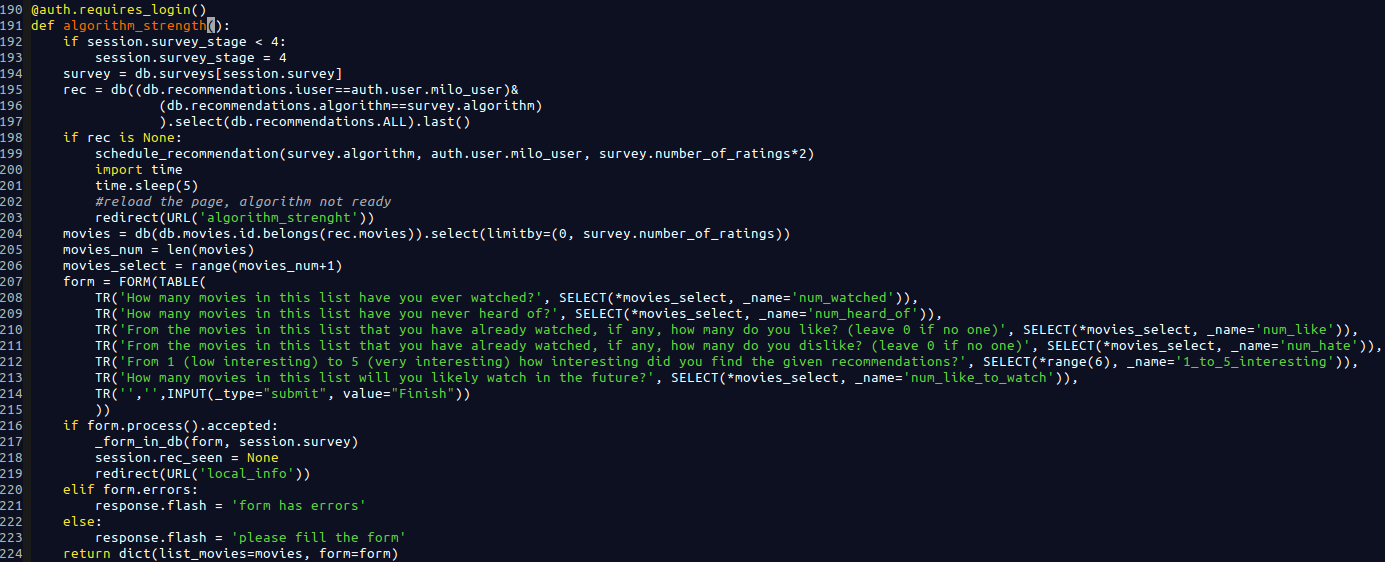
\includegraphics[width=\textwidth]{figures/algorithm_strength.png}
  \caption{Adding new algorithm: algorithm\_strength example}
  \label{fig:algorithm_strength}
\end{figure}

Last lines, from 216 to 224, are for form submission. If the form is recognized to have valid data (accepted) the form data is added to the database using the special \textbf{\_form\_in\_db} function that having a form and a survey id adds the answers that the user provided to the database. Using this function every form created with web2py helpers can be recognized, parsed and stored into database. After saving the data to the database the user is redirected to the last question with the \textit{redirect(URL('local\_info'))} line. Each algorithm type, after processing the data must call this redirect in order to let the user finish the survey.

\section{Crowdsourcing}
\label{sec:crowdsourcing}

Crowdsourcing \cite{crowdsourcing} is a process that involves outsourcing tasks to a distributed group of people. This process can occur both online and offline. The difference between crowdsourcing and ordinary outsourcing is that a task or problem is outsourced to an undefined public rather than a specific body, such as paid employees.

Amazon Mechanical Turk \cite{amazon-mechanical-turk} is a marketplace for work. It gives businesses and developers access to an on-demand, scalable workforce. Workers select from thousands of tasks or \ac{HIT} and work whenever it is convenient. The service has two kind of users: workers and requester.

\begin{itemize}
\item \textbf{Requester}. Asks workers to completer HITs and gets results. Requesters have access to a global 24x7 workforce, get thousands of HITs completed in minutes, and pay only when you are satisfied with the results.
\item \textbf{Worker}. Are the people that perform the HITs. Workers can work from everywhere with an internet connection, choose their work hours and get paid for doing good work.
\end{itemize}

Movish has been designed to work with Amazon Mechanical Turk. After the survey has been created, in the survey list page of figure \ref{fig:surveys_menu}, the administrator has an \textit{Amazon Turk link} which is the link to provide to the Amazon Mechanical Turk interface. The suggested way of integrating Movish with the amazon service is by survey link which is described in their webpage as figure \ref{fig:amazon_turk_survey_link} shows. The administrator has to create a new survey link and use the link provided from the movish admin interface.

\begin{figure}
  \centering
  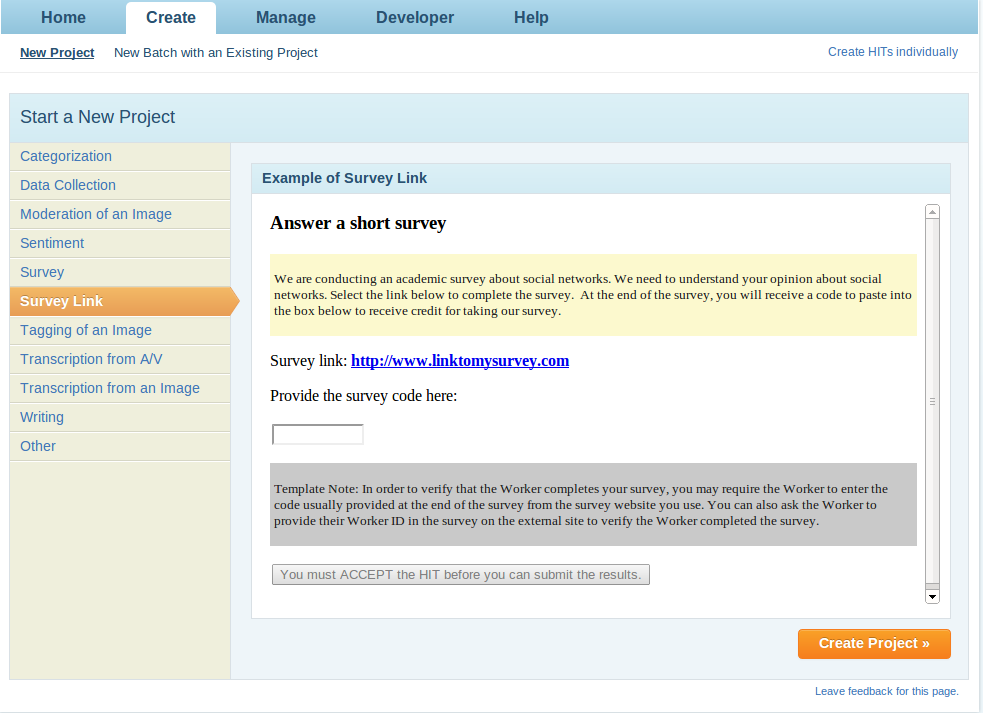
\includegraphics[width=\textwidth]{figures/amazon_turk_survey_link.png}
  \caption{Amazon Mechanical Turk survey link type}
  \label{fig:amazon_turk_survey_link}
\end{figure}

After the HIT has been started from Amazon Mechanical Turk, the administrator can monitor the status of all the HITs from the management console shown in figure \ref{fig:surveys_on_turk}. In that picture the status of the three surveys that I performed during this thesis are shown. We will talk more about them on chapter \ref{chapter:<research_number_of_items>}.
 
\begin{figure}
  \centering
  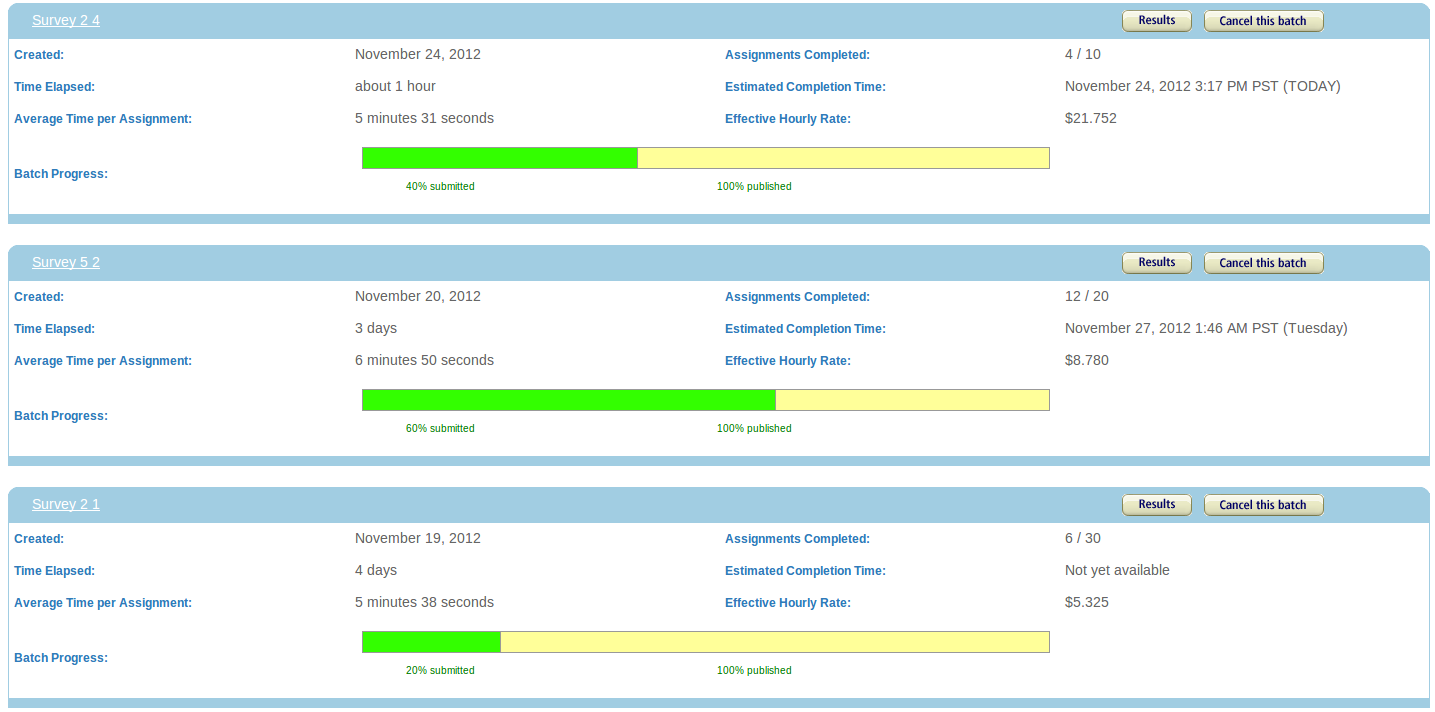
\includegraphics[width=\textwidth]{figures/amazon_turk_surveys.png}
  \caption{Surveys on Amazon Mechanical Turk}
  \label{fig:surveys_on_turk}
\end{figure}

Thanks to the integration with Amazon Mechanical Turk, Movish is able to be a platform to perform surveys without the admin having to worry in promoting the survey which is usually a time consumptive tasks. Based on the amount of work for a survey and the time spent on it (5 minutes and 31 seconds average) the correct pay for a Movish survey HIT is about \$1.50. Having set \$2 as pay for each survey made the system get 10 surveys in less than 3 hours. This has an effective hourly rate for the worker of \$21.687. Having set \$1 as pay for each survey made the system collect 10 surveys after three days with an average of 6 minutes and 56 seconds per survey and an effective hourly rate of \$8.654.

\section{Conclusions}
\label{sec:survey_management_conclusions}

Movish implements a flexible and easy to update survey system. It has being designed in order to support continue modification of the survey types and creation of new surveys. The survey creation has been thought to be performed by an administrator in order to do not modify any line of code. New survey types are easily added with a slightly edit of source code. 
The integration with Amazon Mechanical Turk makes Movish able to also promote itself to reach users thus have completed survey. Using Movish an recommendation system professional can deliver survey without worrying about seeking for users and visibility. 

These features make Movish the best system to deploy survey for recommendation system available today.

\acresetall